\section{Results - Extended model}

\textbf{HUSK AT ÆNDRE Y AKSEN FRA AGE TIL PARTICPATION RATE OF HOURS! PLUS ÆNDRE X-AKSEN TIL age}

To envestigate the results I simulate 200.000 households using the optimal $\beta_L = 24.49$. Using this sample i can do counter factual analysis of households that do get children, and households that do not get children. Figure \ref{fig:ext_model_working_hours} show the average number of working hours of the simulations compared to the true number of hours worked by women. This extended model fits the data considerably better than the simple model, as shown by figure \ref{fig:dqi_model1_average_path_sim_vs_empirical}. Again the models also differ in the action space, where this extended model do not allow for working more than 37 hours a week - the old model did. The average number of hours worked hours is calculated by conditioning on the supplied number of hours working must be above 0. The figure also shows the average number of hours supplied by women when they get children at their specific age. This is true for age 25, 30 and age 35. These households get one child and only one child. For these house holds i do not condition on wether $H>0$. Looking to these households very steep dips in the supplied number of hours are very obvious, at about 5 hours for each of the three age groups. The cohorts of households that get a child at age 30 and 35 year dip to a permanently lower number of supplied hours, where as the cohort that get a child at age 25, get an initial dip, but do at after a certain period of time readjust the number of supplied hours. For all three cohorts the initial dip when the housholds get the child is about 5 hours.

\begin{figure}
    \centering
    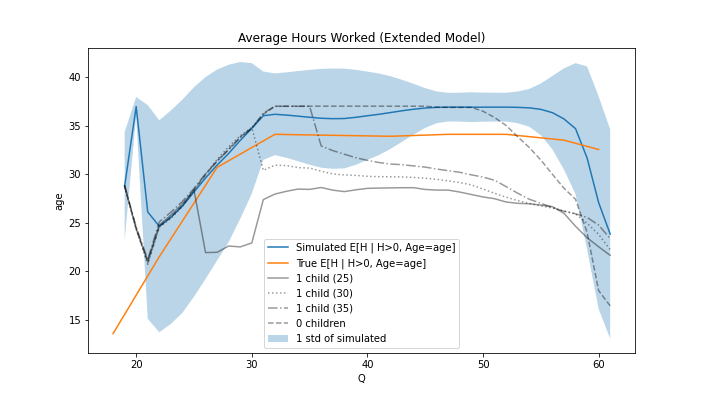
\includegraphics[scale=0.4]{figures/extended_model_average_hours.png}
    \caption{Extended Model Working Hours - Empirical Vs. Simulated}
    \label{fig:ext_model_working_hours}
\end{figure}

Figure \ref{fig:ext_model_particpation_rates} shows the participation rate over the life cycle. The average participation of all simulations is $81.7 \%$ letting the overall number of women out of the workforce be equal to $18.3$ comparing to the the number used for the estimation of $\beta_L$ which was $15 \%$, must be considered a good fit. I have not found good data from Statistics Denmark showing women's average participation rate over the life cycle, implying it's hard for to make inference over the participation rate over the life cycle. However a couple of things can be noted. First and foremost the simulations show a downward sloping trend of participation rates over the life cycle. \textcite{grimm_labour_2001} have investigated female labour participation rate in France over the life cycle. The data  they present suggest that picture is not totally unrealistic. Certain things should however be noted. Their sample ends in 1998, and looking to that data, the downward sloping trend do seem to be pronounced comparing to earlier generations. I have shown four different cohorts in the same image. As before i have focused on families getting 0 children, a cohort of households getting a child at age 25, a cohort of households getting a child at age 30, and lastly a cohort of households getting their first and only child at age 35. The picture is clear, when the child is born, it has a very strong effect on participation rate. The households getting a child at age 25, do seem to have a penalty of 30 percent reduction in participation rate for the next five years.
Families getting their child at age 39 experience a reduction in participation rate of 20 percent, and at last the cohort of households getting a child at age 35 experience a reduction in participation rate at around 10 percent.

\begin{figure}
    \centering
    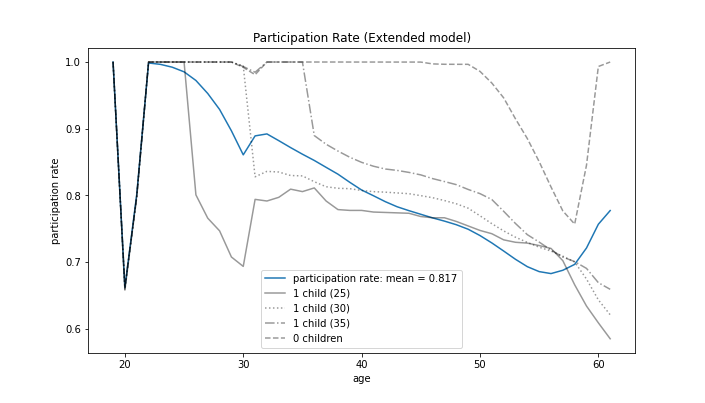
\includegraphics[scale=0.4]{figures/extended_model_participation_rates.png}
    \caption{Participation rates}
    \label{fig:ext_model_particpation_rates}
\end{figure}

Figure \ref{fig:ext_model_impact_earnings_hours} and \ref{fig:ext_model_impact_participation_wage} displays event graphs of households getting a (single) child at different ages. These are normalized against a bench mark - the women of households that do not get children. These event graphs compares to the event graphs by \textcite{kleven_children_2019}, however there a couple of differences. \textcite{kleven_children_2019} considers the husband of the household as benchmark whereas I consider women of households with no children the benchmark. The husband of the household, in this model, is considered to follow a deterministic path, and household heterogeneity only comes from the different choices of the woman of the household, letting this be a more natural comparison for this model. Comparing the results, even though the benchmarks do diverge, does lead to surprisingly similar conclusions. First notice that the earnings do seem to have the largest reduction for households that get children at an early age. The same goes for hours worked, participation rates and wage rates. Secondly the long run penalties do converge to approximately the same levels. Table \ref{tab:extended_results} lists the different long run penalties compared to \textcite{kleven_children_2019}. Comparing the long run penalties, this analysis find 5 percentage points lower long run penalties for earnings, 10 percentage points higher penalty for hours works, 8 percentage points higher penalties for participation rates and 14 percentage points lower penalty for wage rates in this model than the results found by \textcite{kleven_children_2019}.

\begin{figure}[ht]
\begin{subfigure}{.5\textwidth}
  \centering
  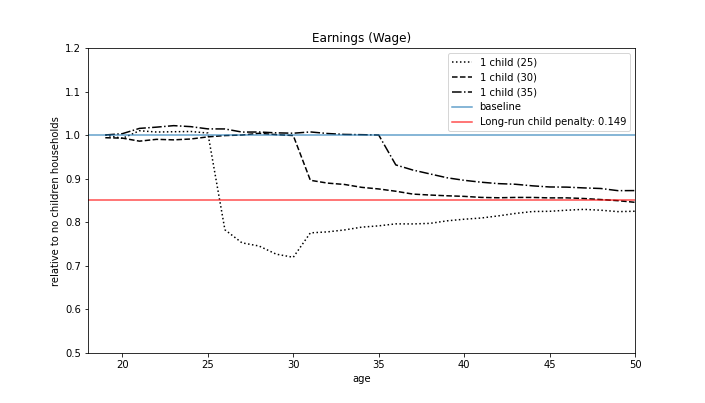
\includegraphics[width=1\linewidth]{figures/extended_model_event_earnings.png}
  \caption{Earnings}
  \label{fig:ext_model_event_earnings}
\end{subfigure}%
\begin{subfigure}{.5\textwidth}
  \centering
  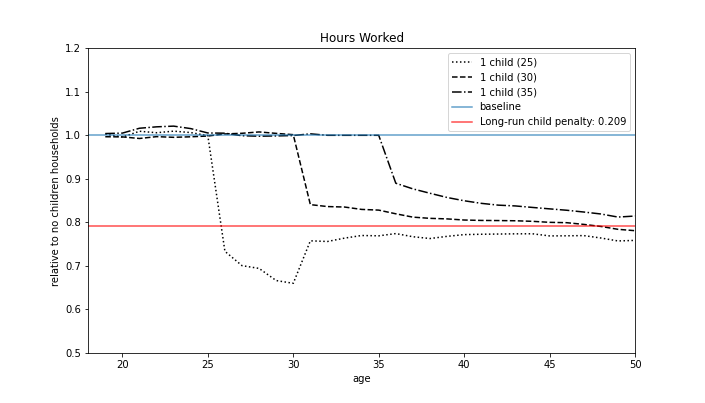
\includegraphics[width=1\linewidth]{figures/extended_model_event_hours_worked.png}
  \caption{Hours Worked}
  \label{fig:ext_model_event_hours}
\end{subfigure}
    \caption{Impact of Children (Earnings and Worked Hours)}
    \label{fig:ext_model_impact_earnings_hours}
\end{figure}

\begin{figure}[ht]
\begin{subfigure}{.5\textwidth}
  \centering
  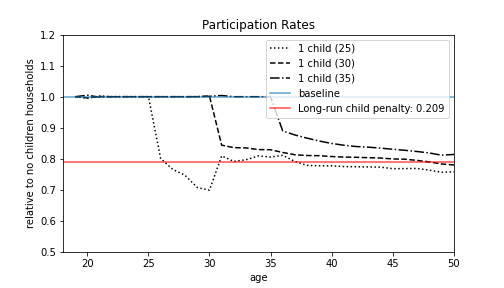
\includegraphics[width=1\linewidth]{figures/extended_model_event_participation_rates.png}
  \caption{Participation Rates}
  \label{fig:ext_model_event_partipation}
\end{subfigure}%
\begin{subfigure}{.5\textwidth}
  \centering
  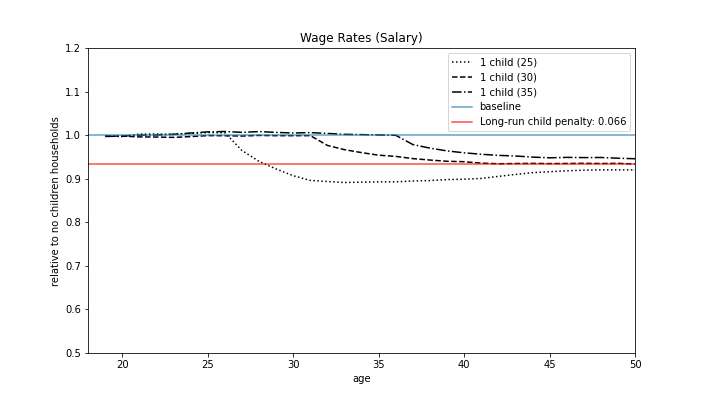
\includegraphics[width=1\linewidth]{figures/extended_model_event_wage_rates.png}
  \caption{Wage Rates}
  \label{fig:ext_model_event_wage_rates}
\end{subfigure}
    \caption{Impact of Children (Participation Rates and Wage Rates)}
    \label{fig:ext_model_impact_participation_wage}
\end{figure}


\textcite{kleven_children_2019} writes that their event graphs of wage rates and hours worked is conditioned on labour market participation. Figure \ref{fig:ext_model_impact_alt} shows these event graphs. Here I find the reverse picture, such that the wage rates and hours worked increase on average when a child is born. This effect must be consequence of selection effects. In other words, this model primarily finds effects, by letting women select out of the labour market, if they are not on high income trajectories of their income path. This clash with the results found by \textcite{kleven_children_2019}. The RHS column of table \ref{tab:extended_results} shows the long run penalties, conditioning on labour market participation.


\begin{figure}[ht]
\begin{subfigure}{.5\textwidth}
  \centering
  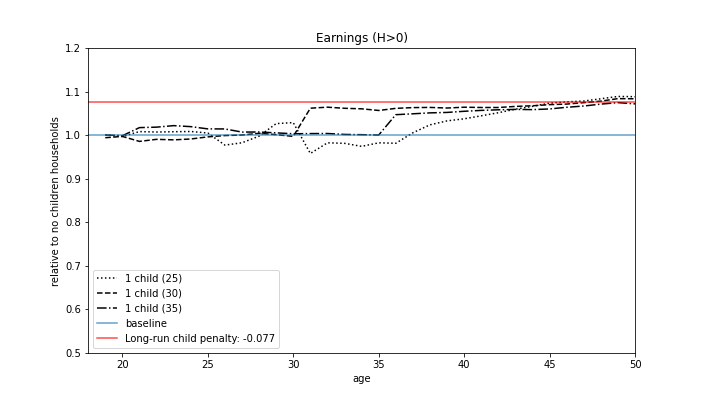
\includegraphics[width=1\linewidth]{figures/extended_model_event_earnings_H>0.png}
  \caption{Earnings Conditional on $H > 0$}
  \label{fig:ext_model_event_earnings_alt}
\end{subfigure}%
\begin{subfigure}{.5\textwidth}
  \centering
  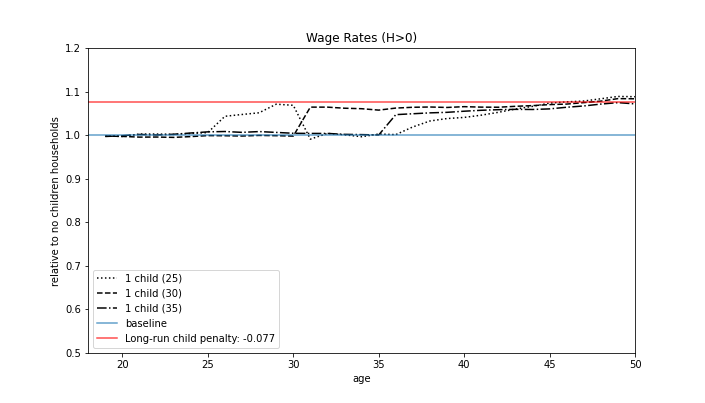
\includegraphics[width=1\linewidth]{figures/extended_model_event_wage_rates_H>0.png}
  \caption{Wage Rates Conditional on $H>0$}
  \label{fig:ext_model_event_wage_rates_alt}
\end{subfigure}
    \caption{Impact of Children conditional on $H>0$}
    \label{fig:ext_model_impact_alt}
\end{figure}

Multiple issues can be attributed to cause these discrepancies between the model presented in this paper and the results found by \textcite{kleven_children_2019}? First, it cannot be rejected that in real danish registry data, labour market participation is defined in less naive way, than it is in this paper. This paper simply assumes, that if a woman supplies zero hours of work $H=0$ then said woman is unemployed. Danish registry data have a more intricate way to ascribe unemployment status to individuals, than just looking at the number of hours worked by an individual, implying that some individuals of the sample in \textcite{kleven_children_2019} are working 0 hours. Secondly this model naively assumes an idiosyncratic wage path following a random walk, this might also contribute to the issues. In general, I believe, that to more accurately find comparable results to \textcite{kleven_children_2019} then the model, should contain more intricate family characteristics, endogenous male labour supply, a more elaborate labour market with multiple sectors etc. However as shown in this paper, using deep reinforcement learning for solving dynamic models, this should be feasible.

\begin{table}[ht]
    \centering
    \begin{tabular}{lrrr}
\toprule
                     &  Kleven et al. &  result &  result (H > 0) \\
\midrule
            Earnings &          0.194 &   0.149 &          -0.077 \\
        Hours worked &          0.097 &   0.209 &           0.000 \\
 Participation rates &          0.130 &   0.209 &             NaN \\
          Wage rates &          0.194 &   0.066 &          -0.077 \\
\bottomrule
\end{tabular}

    \caption{Long run penalties comparison}
    \label{tab:extended_results}
\end{table}




